\begin{frame}
\frametitle{Position vectors}

  \begin{itemize}
   \item Vector $\textbf{u}$: \\
      set of displacement vectors with given direction and magnitude

    \item  Magnitude of $\textbf{u}$: common given magnitude.

    \item Direction of $\textbf{u}$: common given direction, if non-zero magnitude.

    \item Set of zero displacement vectors = zero vector, $\textbf{0}$. \pause

    \item Representative for $\textbf{u}$: \\
      displacement vector $\textbf{AB}$ with the same direction and magnitude

\begin{figure}[h]
  \psfrag{A}{$A$}
  \psfrag{B}{$B$}
  \psfrag{C}{$C$}
  \psfrag{D}{$D$}
  \psfrag{E}{$E$}
  \psfrag{F}{$F$}
  \psfrag{u}{$\textbf{u}$}
  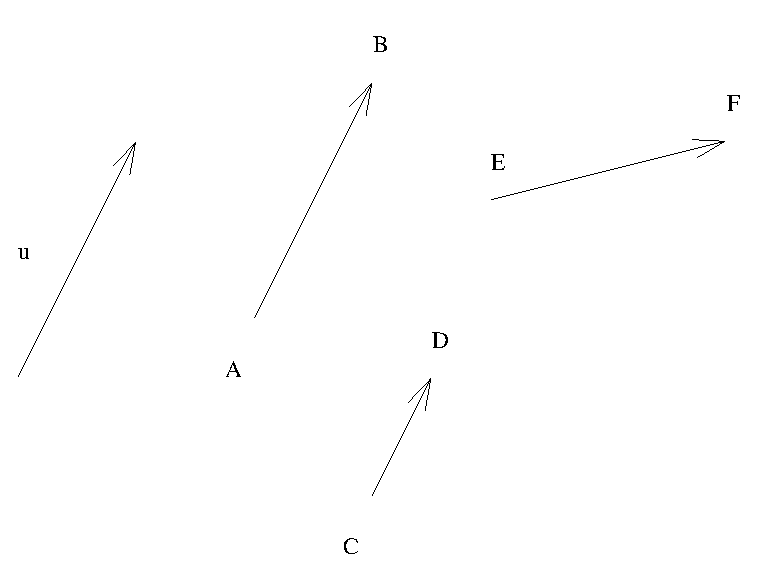
\includegraphics[height=1in]{../../modules/vectors/pictures/ok-vector_representatives.eps}
  \label{fig:vector_representative}

\end{figure}

    \item Intuitive notation:  $\textbf{u}=\textbf{AB}$.

    \item Graphical representation: arrow without fixed tail and head.

    %\item Major advantage: we can translate displacement vectors.
  \end{itemize}
\end{frame}